\documentclass[a4paper,10pt]{article}

\usepackage[utf8]{inputenc}
\usepackage[margin=2.5cm]{geometry}
\usepackage{graphicx}
\usepackage{hyperref}
\usepackage{listings}
\usepackage{xcolor}
\usepackage{fancyhdr}
\usepackage{titlesec}
\usepackage{tcolorbox}
\usepackage{amsmath}
\usepackage{float}
\usepackage{subcaption}
\usepackage{multirow}
\usepackage{cite}

% Configure code listings
\lstset{
    basicstyle=\ttfamily\small,
    backgroundcolor=\color{gray!10},
    frame=single,
    breaklines=true,
    showstringspaces=false,
    commentstyle=\color{green!60!black},
    keywordstyle=\color{blue},
    stringstyle=\color{red}
}

% Configure headers and footers
\setlength{\headheight}{14.49998pt}
\addtolength{\topmargin}{-2.49998pt}
\pagestyle{fancy}
\fancyhf{}
\rhead{SoftEther VPN Lab Activity}
\lhead{Politecnico di Torino}
\cfoot{\thepage}

\title{SoftEther VPN Lab Activity\\
\large Virtual Private Networks Across the Internet}
\author{Renato Mignone\\
\small Student ID: s336973\\
\small MSc in Cybersecurity Engineering\\
\small Politecnico di Torino}

\begin{document}

% Custom title page
\begin{titlepage}
\centering

% Top spacing
\vspace*{2cm}

% University logo

\includegraphics[width=0.4\textwidth]{../resources/General/polito_logo.png}

\vspace{1.5cm}

% Main title
{\Huge \textbf{SoftEther VPN Lab Activity}}

\vspace{0.5cm}

% Subtitle
{\LARGE Virtual Private Networks Across the Internet}

\vspace{1cm}

% Horizontal line
\rule{\textwidth}{1pt}

\vspace{2cm}

% Author information
{\Large \textbf{Renato Mignone}}

\vspace{0.5cm}

{\large Student ID: s336973}

\vspace{1cm}

{\large MSc in Cybersecurity Engineering}

\vspace{0.5cm}

{\large Politecnico di Torino}

\vspace{2cm}

\vfill

% Bottom text
{\small Network and Cloud Security Practical Activity}

\end{titlepage}

% License page
\section*{License}

This work is licensed under a Creative Commons Attribution-NonCommercial-ShareAlike 3.0 Unported License.\\

\noindent
\textbf{You are free:}
\begin{itemize}
    \item \textbf{to Share:} to copy, distribute and transmit the work
    \item \textbf{to Remix:} to adapt the work
\end{itemize}

\textbf{Under the following conditions:}
\begin{itemize}
    \item \textbf{Attribution:} you must attribute the work in the manner specified by the author or licensor (but not in any way that suggests that they endorse you or your use of the work).
    \item \textbf{Noncommercial:} you may not use this work for commercial purposes.
    \item \textbf{Share Alike:} if you alter, transform, or build upon this work, you may distribute the resulting work only under the same or similar license to this one.
\end{itemize}

More information on the Creative Commons website.

\section*{Acknowledgments}

The author would like to thank Professor Daniele Bringhenti, Professor Fulvio Valenza, Professot Gianmarco Bachiorrini and the Politecnico di Torino for providing the foundational knowledge and laboratory environment that made this work possible.


\newpage

% Table of contents
\tableofcontents
\thispagestyle{empty}
\newpage

% Main content
\newpage

\section{Introduction}

This Project involves the implementation and analysis of \textbf{Virtual Private Networks} (VPNs) using \textbf{SoftEther VPN} technology across an Internet infrastructure. VPNs are fundamental network security technologies that provide secure connectivity across shared, potentially untrusted networks by creating encrypted tunnels that preserve the confidentiality, integrity, and authenticity of data transmission.

\noindent
\\
The objective of this lab is to demonstrate how modern VPN technologies can establish secure communication channels between geographically separated networks, mimicking real-world scenarios in which branch offices or remote users need secure access to corporate resources. Through practical implementation, we will examine two different VPN protocols: IPSec and TLS/SSL, comparing their different approaches and methods to achieve network security.

\subsection{Laboratory Objectives}

The main objectives of this lab activity are:

\begin{itemize}
    \item \textbf{VPN Basics:} Learn the essentials of Virtual Private Networks and their application in modern network security architectures.
    
    \item \textbf{SoftEther VPN Deployment:} Install and deploy SoftEther VPN server to utilize multi-protocol VPN services, as IPSec and TLS-based connections.
    
    \item \textbf{Network Topology Design:} Design a realistic network topology using GNS3 that simulates Internet interconnectivity between two remote sites over an ISP infrastructure.
    
    \item \textbf{Protocol Comparison:} Contrast and compare different VPN protocols (IPSec vs. TLS) in terms of security features and complexity.
    
    \item \textbf{Traffic Analysis:} Perform packet capture with Wireshark to observe how differently the VPN protocols encapsulate and protect network traffic differently.
    
    \item \textbf{Security Assessment:} Examine the security mechanisms provided by each VPN implementation, including encryption, authentication, and integrity protection.
\end{itemize}

\subsection{Laboratory Environment and Network Topology}

This lab simulates a scenario in which two geographically separated private networks need to commmunicate securely over the Internet. The topology consists of:

\begin{itemize}
    \item \textbf{Server Site:} A private network (10.0.1.0/24) hosting the SoftEther VPN server
    \item \textbf{Client Site:} A remote private network (10.0.2.0/24) with VPN client capability
    \item \textbf{Internet Infrastructure:} Simulated ISP network providing connectivity between the sites
    \item \textbf{VPN Gateways:} Edge routers providing NAT and routing capabilities, to which a public IP address is assigned
\end{itemize}

\noindent
The configuration demonstrates how VPN technology facilitates secure site-to-site connections, allowing hosts whithin different private networks to communicate as if connected to the same local network, while preserving security attributes across the untrusted Internet infrastructure.

\subsection{System Requirements}

In order to successfully complete this lab activity, the following system requirements must be met:

\begin{tcolorbox}[colback=blue!5!white,colframe=blue!75!black,title=System Requirements]
\textbf{Operating System:}
\begin{itemize}
    \item Linux distribution (Ubuntu 20.04 LTS or newer recommended)
    \item Administrative (sudo) privileges required
\end{itemize}

\textbf{Software Requirements:}
\begin{itemize}
    \item \textbf{GNS3:} Graphical Network Simulator-3, a network simulation platform for simulating realistic network topologies
    \item \textbf{Docker:} Container system for VPN endpoints
    \item \textbf{Wireshark:} Network protocol analyzer
\end{itemize}

\textbf{Hardware Requirements:}
\begin{itemize}
    \item At least 4GB RAM (8GB highly recommended for high performance)
    \item 20GB free disk space
    \item Network interface with Internet connectivity
\end{itemize}
\end{tcolorbox}

\noindent
\textbf{Software Installation:}

\noindent
The following commands can be used to install the necessary software on Ubuntu/Debian systems:

\begin{lstlisting}[language=bash]
# Install GNS3 and dependencies
sudo apt install gns3-gui gns3-server

# Install Docker
sudo apt install docker.io

# Install network analysis tools
sudo apt install wireshark

# Add user to required groups
sudo usermod -aG docker $USER
sudo usermod -aG wireshark $USER
\end{lstlisting}

Note: An install and login cycle may be required after installation in order for group membership changes to take effect. The VPN client programs (strongSwan for IPSec and OpenVPN for TLS) will be pre-installed inside the Docker containers during lab setup.

\subsection{Lab Structure}

The report is organized into these sections:

\begin{enumerate}
    \item \textbf{Theoretical Background:} Introduction to VPN technologies, SoftEther VPN architecture, and employed security protocols.
    
    \item \textbf{Network Topology:} Schematic network description employed during simulation and IP addressing strategy.
    
    \item \textbf{Initial Configuration:} Setup of the GNS3 environment, the routers, and the container infrastructure.
    
    \item \textbf{SoftEther VPN Server:} Installation of the VPN server with multi-protocol support.
    
    \item \textbf{IPSec Configuration:} StrongSwan-based IPSec-based VPN implementation.
    
    \item \textbf{TLS Configuration:} OpenVPN client-based TLS/SSL VPN implementation.
        
\end{enumerate}

Each section contains in-practice implementation steps, configuration examples, and result analysis, providing a thorough overview of VPN technologies and applications in real-world contexts.


\newpage

\section{Theoretical Background}

This chapter gives the theoretical background necessary to understand the Virtual Private Network technologies employed in this lab. We cover the fundamentals of VPNs, the specific architectures of SoftEther VPN, and the security protocols that enable the secure communication over untrusted networks.

\subsection{Virtual Private Networks (VPNs)}

Virtual Private Networks are network security solutions that provide connectivity utilizing shared infrastructure while maintaining properties typically offered in private networks. VPNs create secure communication channels over potentially untrusted networks by implementing various security mechanisms at different layers of the network stack.\\

\noindent
\textbf{Core VPN Properties:}

\noindent
A VPN must provide some essential properties to enable secure communication:

\begin{itemize}
    \item \textbf{Data Confidentiality:} Encryption algorithms protect data content from unauthorized access during transmission over public networks.
    
    \item \textbf{Data Integrity:} Cryptographic hash functions and message authentication codes ensure that data has not been modified during transmission.
    
    \item \textbf{Authentication:} Both peer authentication (verification of communicating endpoints's identities) and data origin authentication are essential for secure VPN operation.
    
    \item \textbf{Access Control:} VPN policies determine which traffic is permitted and how it needs to be processed.
    
    \item \textbf{Anti-Replay Protection:} Sequence numbers and time stamps prevent malicious replay of previously captured packets.
\end{itemize}

\noindent
\textbf{VPN Classification:}

\noindent
VPNs can be classified based on their method of implementation and the network layers at which security is enforced. The layers considered in this lab are:

\begin{itemize}
    \item \textbf{Network Layer VPNs:} Operate at the IP layer (L3), e.g. IPSec-based ones
    \item \textbf{Transport Layer VPNs:} Implement security at L4, e.g. TLS/SSL VPNs
\end{itemize}

\subsection{SoftEther VPN Architecture}

SoftEther VPN represents a unique approach to VPN deployment with a unified platform to support multiple VPN protocols simultaneously \cite{softether_official}. This feature of multi-protocol support enables straightforward comparison and evaluation of different VPN technologies in a single deployment.

\begin{figure}[H]
\centering
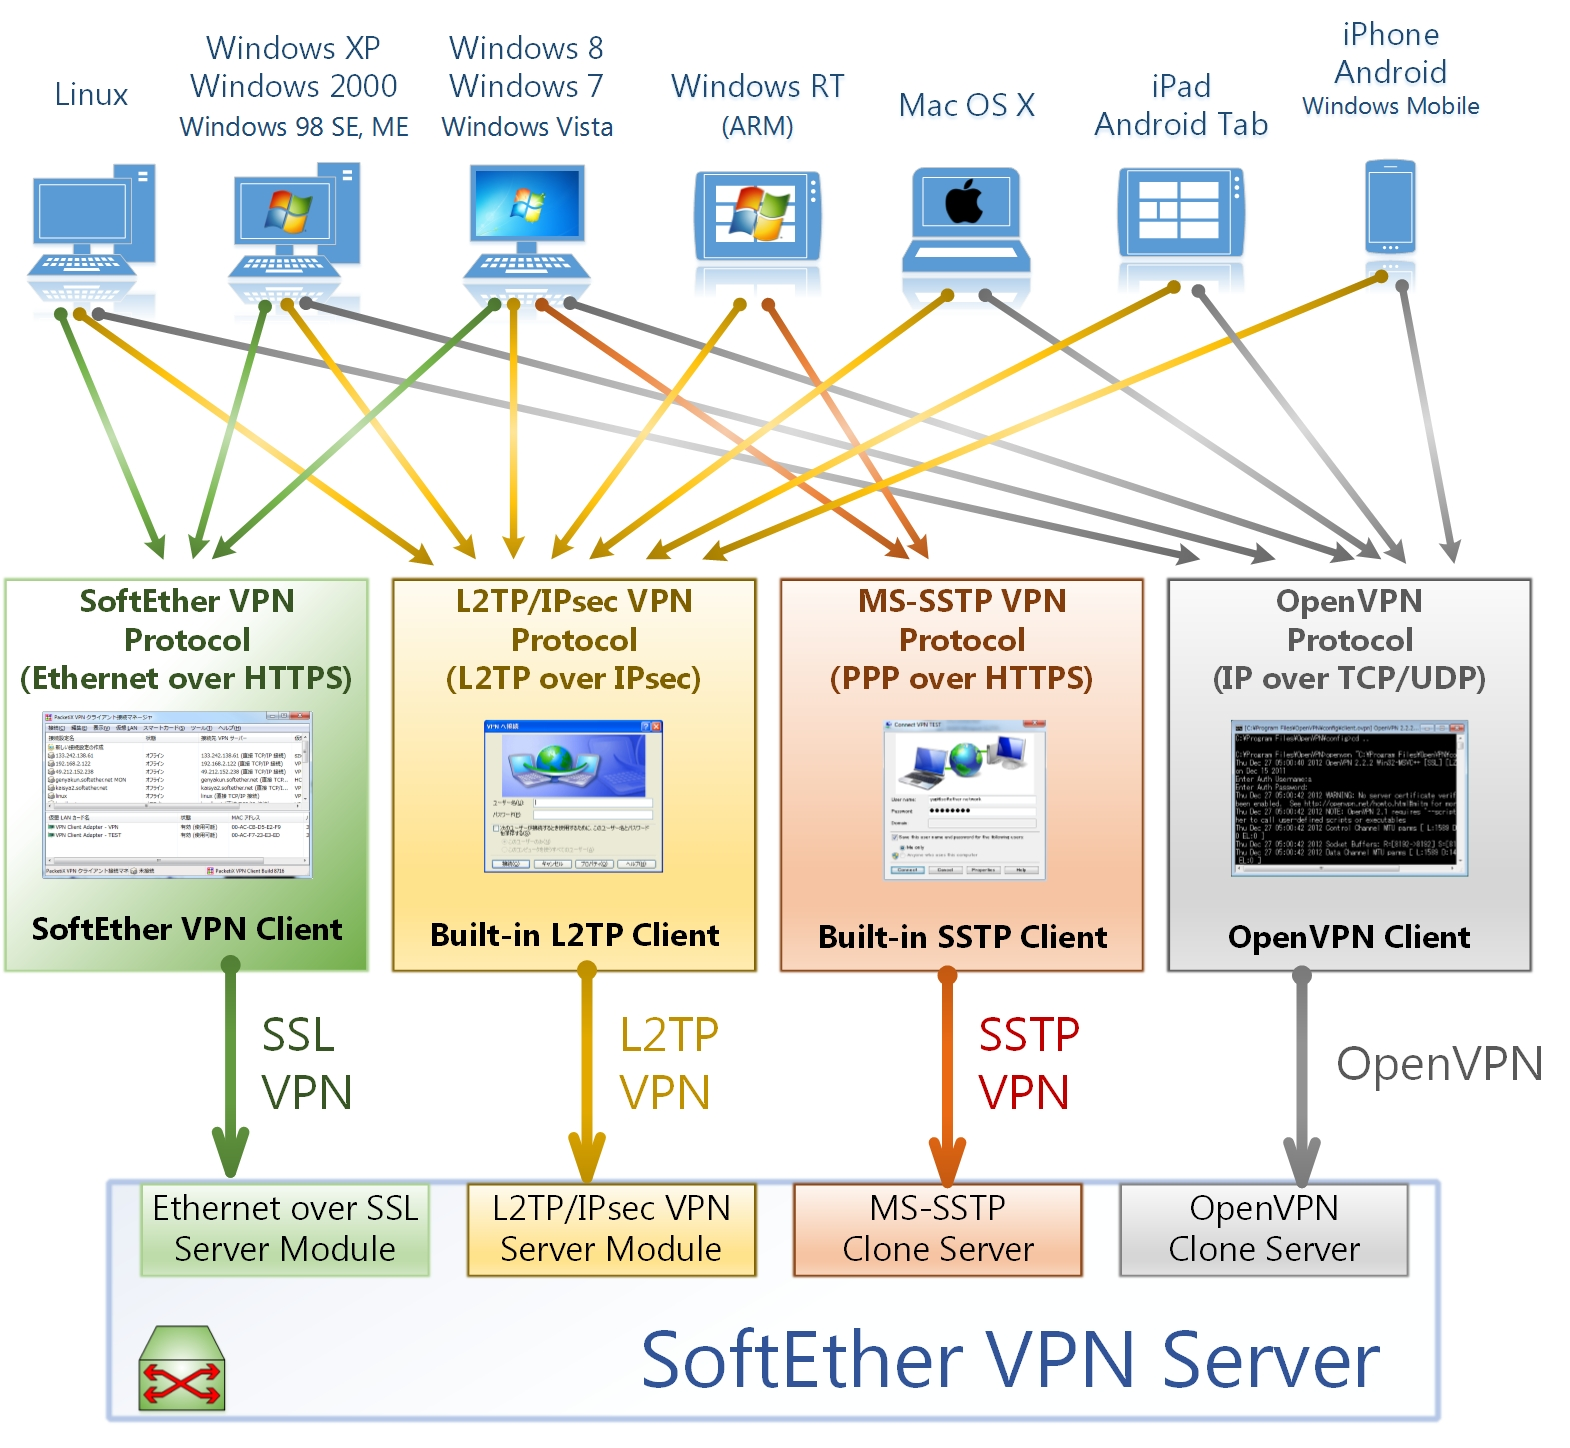
\includegraphics[width=0.4\textwidth]{../resources/Images/SoftEther_VPN_Architecture.jpg}
\caption{SoftEther VPN Multi-Protocol Architecture}
\label{fig:softether_architecture}
\end{figure}

As indicated in Figure \ref{fig:softether_architecture}, SoftEther VPN's architecture reflects its adaptability in the sense of offering Multiple client operating systems and VPN protocols. The figure explains how different hosts with different operating systems can connect to a single SoftEther VPN Server using different VPN protocols:

\begin{itemize}
    \item \textbf{SoftEther VPN Protocol:} Ethernet over HTTPS Proprietary protocol
    \item \textbf{L2TP/IPSec VPN Protocol:} Common L2TP over IPSec implementation
    \item \textbf{MS-SSTP VPN Protocol:} Microsoft's Secure Socket Tunneling Protocol using PPP over HTTPS
    \item \textbf{OpenVPN Protocol:} SSL/TLS-based VPN using IP over TCP/UDP
\end{itemize}

\noindent
\\
\textbf{Multi-Protocol Support:}

\noindent
SoftEther VPN's architecture relies on \textit{protocol abstraction}, where different VPN protocols are realized as modules within a common framework. The key protocols that we will use in this lab are:

\begin{itemize}
    \item \textbf{IPSec Support:} Built in support for both AH (Authentication Header) and ESP (Encapsulating Security Payload) protocols in tunnel mode
    \item \textbf{SSL/TLS Support:} Built-in TLS server compatible with OpenVPN clients and other SSL VPN solutions
\end{itemize}

\noindent
\textbf{Virtual Hub Architecture:}

\noindent
The core of SoftEther VPN is the Virtual Hub concept, which acts as a virtual Ethernet switch. This architecture facilitates the aggregation of multiple VPN sessions of different protocols, provides strong routing and bridging capabilities, and accomodates centralized policy enforcement and logging. Building complex network topologies, including both site-to-site networks and remote access networks, is also supported by the Virtual Hub and thus is a valuable component of SoftEther VPN applications.

\noindent
\\
\textbf{SecureNAT Functionality:}

\noindent
SoftEther VPN comes with a Built-in NAT (Network Address Translation) and DHCP server feature named SecureNAT, which is employed to make it easy to set up VPN clients by

\begin{itemize}
    \item Automatically assigning IP addresses to VPN clients
    \item Providing DNS resolution services
    \item Providing Internet access for VPN clients through NAT
\end{itemize}

\subsection{IPSec Protocol Suite}

Internet Protocol Security (\textbf{IPSec}) is a suite that provides security at the IP layer by adding headers to IP packets \cite{rfc4301}. It may operate in transport mode (only securing payload) or tunnel mode (encapsulating the entire packet). IPSec implementations have been the subject of extensive cryptographic analysis \cite{ferguson_ipsec} and are standardized by various bodies, like NIST \cite{nist_vpn_guide}.

\noindent
A key part is the \textbf{Encapsulating Security Payload} (ESP), which ensures confidentiality by encrypting packets and provides optionally integrity and authentication as well. ESP in tunnel mode, encrypts the whole IP packet, creating new IP headers for the routing. \textbf{Security Associations} (SAs) are agreements between peers that specify parameters as encryption algorithms, keys, and endpoints; each of them is associated with a Security Parameter Index (SPI). Their manual management is usually controlled by Internet Key Exchange protocols: IKEv1 (with main and aggressive modes) and IKEv2 (which both improves performance and security). In this project, IPSec (via ESP, SA, and IKE) is used to establish an encrypted network layer tunnel for situations where protection at the kernel level is required for packets.

\subsection{TLS/SSL for VPN Implementation}

\textbf{Transport Layer Security} (TLS) provides session-layer security though a handshake to agree on cipher suites \cite{rfc8446}. TLS-based VPNs (such as \textbf{OpenVPN}), tunnel arbitrary IP traffic in a TLS channel \cite{openvpn_official}, leveraging the widespread availability of TLS support and negotiable cipher suites. This approach places security processing in user space, which may be easier to deploy and customize, but with some performance trade-offs compared to kernel-based solutions.

\textbf{Layers of Authentication of TLS VPNs:} Care must be taken to distinguish between TLS handshake authentication (typically server certificate verification) and application-layer authentication occurring inside the established TLS tunnel. User credentials are transmitted as application data after the secure channel has been established, again controlling access beyond the transport-layer security.

\subsection{Client-Side VPN Technologies}

\textbf{StrongSwan (IPSec):}

\noindent
strongSwan is an open-source IPSec implementation used in this project for establishing and maintaining IPSec tunnels \cite{strongswan_official, strongswan_docs}. It supports IKEv1 and IKEv2, a cryptographic algorithm set, and other features like NAT traversal \cite{rfc3948}. It can be configured with simple files (e.g., \texttt{ipsec.conf} and \texttt{ipsec.secrets}), and it supports the Linux kernel’s IPSec stack. In our setup, strongSwan handles automatic key exchanges and maintains SAs for secure network-layer tunnels.\\

\noindent
\textbf{OpenVPN Client (TLS):}

\noindent
OpenVPN is the TLS-based client solution in this project \cite{openvpn_official, openvpn_howto}. It is based on OpenSSL for cryptography \cite{openssl_project}, supports both UDP and TCP transports, and can be configured in tun (Layer 3) or tap (Layer 2) mode. Certificate-based authentication using a certificate ensures that only authorized endpoints connect. OpenVPN’s user-space implementation supports flexible scripting hooks and logging, so it is easily adapted to custom remote-access applications in the lab.

\subsection{Comparative Analysis Framework}

Having theoretical knowledge of the differences between IPSec and TLS implementations, provides the basis for effective comparison:

\begin{itemize}
    \item \textbf{Architecture Differences:} IPSec is implemented at the network layer (typically in kernel space), whereas TLS-based VPNs run in user space at the session layer.
    
    \item \textbf{Performance Considerations:} IPSec generally has lower overhead with kernel integration; TLS-based VPNs offer more flexibility but may have more user space processing.
    
    \item \textbf{Deployment Complexity:} IPSec configurations may be more complex but follow broadly enstablished standards, while TLS-based VPNs like OpenVPN are more likely to have simpler initial setup and greater customizability.
    
\end{itemize}


This conceptual foundation establishes the necessary knowledge for understanding the actual application and comparison of SoftEther VPN's multi-protocol capabilities in subsequent parts of this lab activity.
\newpage

\section{Network Topology and Architecture}

This section presents the network topology designed for the SoftEther VPN laboratory activity. The implementation simulates a realistic scenario where two geographically separated private networks communicate securely across the Internet through VPN tunnels. 

\subsection{Topology Overview}

The laboratory network topology consists of five main components that work together to create a realistic Internet-based VPN scenario:

\begin{figure}[H]
\centering
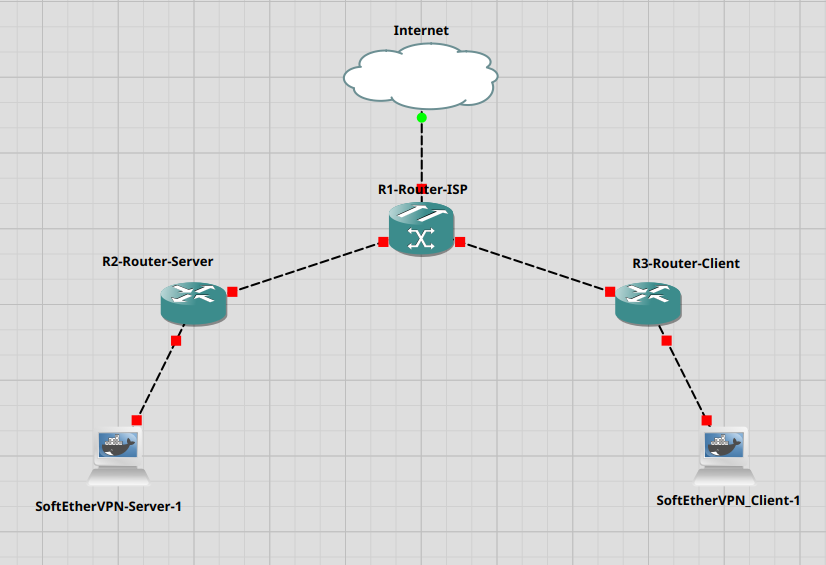
\includegraphics[width=0.9\textwidth]{../resources/Images/GNS3_Structure.png}
\caption{GNS3 Network Topology - VPN Across the Internet}
\label{fig:gns3_topology}
\end{figure}

The network architecture follows an end-to-end VPN design where:

\begin{itemize}
    \item \textbf{Server Site:} Contains the SoftEther VPN server hosted within a private network
    \item \textbf{Client Site:} Represents a remote branch office requiring VPN connectivity
    \item \textbf{Internet Infrastructure:} Simulated ISP network providing public connectivity
    \item \textbf{Edge Routers:} Perform NAT and routing functions, providing Internet connectivity for the private networks
    \item \textbf{VPN Endpoints:} Docker containers hosting the actual VPN software (server and client)
\end{itemize}

This topology effectively demonstrates how end-to-end VPN technology enables secure communication between hosts in different private networks across untrusted public infrastructure, representing common real-world deployment scenarios where VPN software runs directly on the endpoints rather than on gateway devices.

\subsection{IP Addressing Scheme}

The network addressing scheme uses a combination of private and public IP addresses to simulate realistic Internet connectivity. The addressing follows RFC standards for private addressing (RFC 1918) and uses documentation addresses (RFC 5737) for public IP simulation.

\begin{table}[H]
\centering
\caption{Network Interface Configuration}
\label{tab:ip_addressing}
\begin{tabular}{|l|l|l|l|}
\hline
\textbf{Device} & \textbf{Interface} & \textbf{IP Address} & \textbf{Description} \\
\hline
\multirow{2}{*}{Router 2 (Server-side)} & LAN (Fa0/0) & 10.0.1.1/24 & Private Network 1 \\
 & WAN (Fa0/1) & 203.0.113.1/24 & Public IP (RFC 5737) \\
\hline
\multirow{3}{*}{ISP Router} & Interface Fa0/0 & 203.0.113.254/24 & Connected to Router 2 \\
 & Interface Fa0/1 & 198.51.100.254/24 & Connected to Router 3 \\
 & Interface Fa1/0 & DHCP Assigned & Internet Cloud \\
\hline
\multirow{2}{*}{Router 3 (Client-side)} & WAN (Fa0/1) & 198.51.100.1/24 & Public IP (RFC 5737) \\
 & LAN (Fa0/0) & 10.0.2.1/24 & Private Network 2 \\
\hline
SoftEther Server & eth0 & 10.0.1.2/24 & VPN Server Host \\
\hline
VPN Client & eth0 & 10.0.2.2/24 & VPN Client Host \\
\hline
\end{tabular}
\end{table}

\textbf{Network Segments:}

\begin{itemize}
    \item \textbf{Server Network (10.0.1.0/24):} Private subnet hosting the SoftEther VPN server
    \item \textbf{Client Network (10.0.2.0/24):} Remote private subnet with VPN client
    \item \textbf{ISP Segment 1 (203.0.113.0/24):} Public network between ISP and server-side 
    \item \textbf{ISP Segment 2 (198.51.100.0/24):} Public network between ISP and client-side 
    \item \textbf{VPN Tunnel Networks:} Virtual addressing for VPN connectivity (assigned dynamically)
\end{itemize}

\subsection{Device Roles and Functions}

Each component in the network topology serves a specific purpose in demonstrating VPN functionality:

\subsubsection{ISP Router (R1-Router-ISP)}

The ISP router simulates Internet Service Provider infrastructure and provides:

\begin{itemize}
    \item \textbf{Internet Connectivity:} DHCP-assigned public IP address with MAC address spoofing for network access.
    \item \textbf{Inter-Site Routing:} Routes traffic between the two remote sites through simulated Internet infrastructure
    \item \textbf{NAT Traversal Support:} Enables VPN protocols to function through Network Address Translation
    \item \textbf{Public IP Assignment:} Provides public addressing for both edge routers
\end{itemize}

The ISP router configuration includes static routes for both private networks and implements a default route to the Internet cloud.

\subsubsection{Server-Side Router (R2-Router-Server)}

This edge router connects the server's private network to the Internet and implements:

\begin{itemize}
    \item \textbf{Network Address Translation:} Port Address Translation management
    \item \textbf{VPN Port Forwarding:} Static NAT rules to forward VPN traffic to the server:
    \begin{itemize}
        \item Port 500/UDP: ISAKMP forwarded to SoftEther server
        \item Port 4500/UDP: NAT-T forwarded to SoftEther server
        \item Port 443/TCP: HTTPS/TLS forwarded to SoftEther server
    \end{itemize}
    \item \textbf{Default Gateway:} Routing for the server's private network
    \item \textbf{Transparent Routing:} Routes VPN traffic between Internet and private network without VPN processing
\end{itemize}

\subsubsection{Client-Side Router (R3-Router-Client)}

The client-side edge router provides similar functionality for the remote site:

\begin{itemize}
    \item \textbf{PAT Configuration:} Network address translation for client network connectivity
    \item \textbf{Default Routing:} Internet access for the client private network
    \item \textbf{Transparent VPN Support:} Allows VPN client software to establish connections through NAT without router-based VPN processing
\end{itemize}

\subsubsection{SoftEther VPN Server Container}

The server container runs the SoftEther VPN software with the following configuration:

\begin{itemize}
    \item \textbf{Container Image:} \texttt{siomiz/softethervpn:latest}
    \item \textbf{Multi-Protocol Support:} Simultaneous IPSec and TLS/SSL VPN services
    \item \textbf{Virtual Hub:} DEFAULT hub for client connections
    \item \textbf{User Management:} Configured with test user accounts for VPN authentication
    \item \textbf{Certificate Management:} Self-signed certificates for TLS-based connections
\end{itemize}

\subsubsection{VPN Client Container}

The client container simulates a remote user or branch office with:

\begin{itemize}
    \item \textbf{Container Image:} \texttt{ubuntu:latest}
    \item \textbf{IPSec Client:} StrongSwan software for IPSec connectivity
    \item \textbf{TLS Client:} OpenVPN client for SSL/TLS VPN connections
\end{itemize}

\subsection{Network Communication Flow}

The network design enables several communication scenarios:

\begin{enumerate}
    \item \textbf{Direct Internet Communication:} Both sites can access Internet resources through their respective ISP connections
    
    \item \textbf{End-to-End VPN Tunnel Establishment:} The VPN client container initiates direct VPN connections to the SoftEther server container using either:
    \begin{itemize}
        \item IPSec protocol (strongSwan client to SoftEther server)
        \item TLS/SSL protocol (OpenVPN client to SoftEther server)
    \end{itemize}
    
    \item \textbf{Encrypted Inter-Site Communication:} Once VPN tunnels are established, the client can communicate securely with resources in the server's network
    
    \item \textbf{NAT Traversal:} VPN protocols handle NAT traversal automatically, allowing encrypted tunnels to pass through the edge routers
\end{enumerate}

\subsection{Security Considerations}

The network topology incorporates several security features:

\begin{itemize}
    \item \textbf{Private Addressing:} Internal networks use RFC 1918 private addresses, preventing direct Internet access
    \item \textbf{NAT Protection:} Edge routers provide implicit firewall protection through NAT
    \item \textbf{VPN Encryption:} All inter-site communication is protected by VPN encryption
    \item \textbf{Authentication:} VPN connections require user credentials and/or certificates
    \item \textbf{Protocol Separation:} Different VPN protocols operate on distinct ports for protocol isolation
\end{itemize}

This topology provides a foundation for comparing different VPN implementations while maintaining realistic network security practices and demonstrating practical deployment scenarios.

\newpage

\section{Initial Network Configuration}

This section details the step-by-step process of setting up the laboratory environment, including GNS3 configuration, router setup, and Docker container deployment. The configuration establishes the basic network infrastructure that will support the VPN implementations.

\subsection{GNS3 Environment Setup}

The laboratory utilizes GNS3 (Graphical Network Simulator-3) to create a realistic network topology. GNS3 provides the platform for simulating Cisco routers, Docker containers, and network connectivity required for the VPN demonstration.

\subsubsection{Device Import and Template Creation}

\textbf{Cisco Router Template:}

\noindent
The topology requires Cisco 7200 routers running IOS version 124-24.T5. This specific IOS image is chosen because it represents a freely available alternative to modern commercial Cisco IOS versions. While newer platforms like IOSv (IOS Virtual) offer enhanced features and performance, they require valid Cisco licensing agreements which can be costly for educational purposes. The 124-24.T5 image, although older and not widely deployed in current production environments, provides all the fundamental routing and NAT capabilities required for this laboratory exercise. To import the router template:

\begin{enumerate}
    \item Open GNS3 and click the \textbf{router icon} in the left panel
    \item Select \textbf{"New Template"} at the bottom
    \item Choose \textbf{"Install an appliance from the GNS3 server"}
    \item Filter by \textbf{"CISCO"} and locate \textbf{"Cisco 7200"}
    \item Install the template and select version \textbf{"124-24.T5"}
    \item Import the router image file to complete the setup
\end{enumerate}

\noindent
\textbf{Docker Container Setup:}

\noindent
Two Docker containers are required for the VPN endpoints:

\begin{itemize}
    \item \textbf{Server Container Image:} \texttt{siomiz/softethervpn:latest}
    \item \textbf{Client Container Image:} \texttt{ubuntu:latest}
\end{itemize}

\noindent
To add containers to the GNS3 project:

\begin{enumerate}
    \item Navigate to Edit → Preferences in GNS3
    \item Select "Docker containers" from the left panel
    \item Click "New" to add a container
    \item Enter the image name (e.g., \texttt{siomiz/softethervpn:latest})
    \item Configure the container name and complete the setup
    \item Repeat for the Ubuntu client container
\end{enumerate}

\noindent
You will now see the containers in the left panel of GNS3, ready to be dragged into the workspace. So now you can recreate the same topology as shown in the figure in the section 3 of this document. Clicking on the wire on the left panel, you will be able to connect the devices together, creating the network topology defined. Choose the right interfaces for each connection as shown in the table in the section 3.2.\\

\noindent
\textbf{Important Router Configuration Note:}
\noindent
Before proceeding with the router configurations, you must configure the ISP router to have three interfaces instead of the default two. This is necessary because the ISP router needs to connect to both edge routers and the Internet cloud. To configure the ISP router slots:

\begin{enumerate}
    \item Right-click on the ISP router in GNS3
    \item Select \textbf{"Configure"} from the context menu
    \item Navigate to the \textbf{"Slots"} section in the configuration dialog
    \item Replace the existing slot configuration from \textbf{"C7200-IO-FE"} to \textbf{"C7200-IO-2FE"}
    \item Apply the changes and close the configuration dialog
\end{enumerate}

This configuration change provides the ISP router with three FastEthernet interfaces (Fa0/0, Fa0/1, and Fa1/0) as required by the network topology, allowing it to connect to both edge routers and the Internet cloud simultaneously.

\subsection{Container Configuration}

The Docker containers require specific configuration for persistent storage and network setup.

\subsubsection{Server Container Setup}

The SoftEther VPN server container needs persistent directories for configuration files:

\begin{enumerate}
    \item Open the server container configuration in GNS3
    \item Navigate to Advanced Settings
    \item Add the following additional directory:
    \begin{itemize}
        \item \texttt{/usr/vpnserver}
    \end{itemize}
\end{enumerate}

\noindent
This directory will be created in the GNS3 project folder, allowing persistent storage of configuration files between container restarts.\\

\noindent
\textbf{Server Configuration File Setup:}

\noindent
To ensure the SoftEther VPN server starts with the proper configuration, you must place the \texttt{vpn\_server.config} file in the correct persistent directory:

\begin{enumerate}
    \item Navigate to your GNS3 project directory on the local filesystem
    \item Open the \texttt{project-files} folder
    \item Locate the \texttt{docker} subdirectory
    \item Find the server container folder (usually named after the container)
    \item Navigate to the \texttt{usr/vpnserver} directory within the container folder
    \item Place the \texttt{vpn\_server.config} file in this directory
\end{enumerate}

\noindent
This ensures that when the container starts, the SoftEther VPN service will automatically load the pre-configured settings, including user accounts, IPSec settings, and SSL/TLS configurations.

\subsubsection{Client Container Setup}

The client container requires similar configuration for persistent storage:

\begin{enumerate}
    \item Open the client container configuration in GNS3
    \item Navigate to Advanced Settings  
    \item Add the additional directory: \texttt{/client}
\end{enumerate}

\noindent
\textbf{Client Configuration Files Setup:}

\noindent
The client container requires multiple configuration files for both IPSec and TLS VPN implementations. Place all the following files in the client's persistent directory:

\begin{enumerate}
    \item Navigate to your GNS3 project directory on the local filesystem
    \item Open the \texttt{project-files} folder
    \item Locate the \texttt{docker} subdirectory
    \item Find the client container folder
    \item Navigate to the \texttt{client} directory within the container folder
    \item Place the following files in this directory:
    \begin{itemize}
        \item \textbf{IPSec files:} \texttt{ipsec.conf} and \texttt{ipsec.secrets}
        \item \textbf{TLS/OpenVPN files:} \texttt{softether.ovpn}, \texttt{ca.crt}, and \texttt{credentials.txt}
    \end{itemize}
\end{enumerate}

\noindent
This setup ensures that all necessary VPN client configuration files are available when the container starts, allowing seamless connection to both IPSec and TLS VPN services.

\subsection{Project Startup and Device Access}

Once all configurations are complete and files are properly placed in their persistent directories, you can start the laboratory environment.

\subsubsection{Starting the GNS3 Project}

To start all devices and containers in the project:

\begin{enumerate}
    \item Click the green \textbf{Play button} in the top toolbar of GNS3
    \item This will start all routers and Docker containers simultaneously
    \item Wait for all devices to complete their boot process
    \item Verify that all device icons show a green status indicator
\end{enumerate}

\subsubsection{Accessing Device Terminals}

To interact with the network devices and containers:

\textbf{For Cisco Routers:}
\begin{enumerate}
    \item Right-click on any router device
    \item Select \textbf{"Console"} from the context menu
    \item This opens the router's command-line interface
\end{enumerate}

\noindent
\textbf{For Docker Containers:}
\begin{enumerate}
    \item Right-click on any container (server or client)
    \item Select \textbf{"Auxiliary Console"} from the context menu
    \item This opens the container's terminal interface
    \item Use this terminal for all container-based commands and configurations
\end{enumerate}

\textbf{Important Note:} For Docker containers, always use the "Auxiliary Console" option rather than the regular console, as it provides the proper terminal interface for interacting with the containerized operating system.

\subsection{Router Configuration}

Now that you can access the router terminals, proceed with configuring the three routers with specific configurations to simulate realistic Internet connectivity and routing behavior.

\subsubsection{ISP Router (R1-Router-ISP)}

The ISP router provides Internet connectivity and inter-site routing. The configuration includes interface setup, MAC address spoofing for DHCP, and routing table entries.

\begin{lstlisting}[language=bash]
enable
configure terminal

# Configure interface to Router 2 (Server-side)
interface FastEthernet0/0
  ip address 203.0.113.254 255.255.255.0
  no shutdown
exit

# Configure interface to Router 3 (Client-side)  
interface FastEthernet0/1
  ip address 198.51.100.254 255.255.255.0
  no shutdown
exit

# Configure Internet interface with DHCP and MAC spoofing
interface FastEthernet1/0
  mac-address xxxx.xxxx.xxxx  # Replace with host machine MAC
  ip address dhcp
  no shutdown
exit

# Configure static routes for private networks
ip route 198.51.100.0 255.255.255.0 FastEthernet0/1
ip route 203.0.113.0 255.255.255.0 FastEthernet0/0

# Configure default route to Internet
ip route 0.0.0.0 0.0.0.0 FastEthernet1/0

end
write memory
\end{lstlisting}

\noindent
\textbf{Important Note - MAC Address Spoofing:} 

\noindent
The MAC address spoofing is necessary because the Politecnico di Torino WiFi network's DHCP server implements MAC address filtering for security purposes. Without using the host machine's MAC address, the DHCP server will not assign a valid IP address to the router interface, preventing Internet connectivity for the simulated network. To obtain your host machine's MAC address:

\begin{lstlisting}[language=bash]
# Display all network interfaces and their MAC addresses
ip a

# Look for the active network interface (usually wlan0 for WiFi or eth0 for Ethernet)
# The MAC address appears after "link/ether"
# Example output:
# 2: wlan0: <BROADCAST,MULTICAST,UP,LOWER_UP> mtu 1500 qdisc mq state UP group default qlen 1000
#     link/ether 1c:ce:51:3f:98:20 brd ff:ff:ff:ff:ff:ff
\end{lstlisting}

\noindent
Copy the MAC address from your active network interface and convert it to Cisco format by adding dots every four characters:
\begin{itemize}
    \item \textbf{Linux format:} 1c:ce:51:3f:98:20
    \item \textbf{Cisco format:} 1cce.513f.9820
\end{itemize}

Replace \texttt{xxxx.xxxx.xxxx} in the configuration with your converted MAC address.

\subsubsection{Server-Side Router (R2-Router-Server)}

This router connects the server's private network to the Internet and implements NAT with port forwarding for VPN services.

\begin{lstlisting}[language=bash]
enable
configure terminal

# Configure LAN interface (connected to server)
interface FastEthernet0/0
  ip address 10.0.1.1 255.255.255.0
  ip nat inside
  no shutdown
exit

# Configure WAN interface (connected to ISP)
interface FastEthernet0/1
  ip address 203.0.113.1 255.255.255.0
  ip nat outside
  no shutdown
exit

# Configure static NAT for VPN services
ip nat inside source static udp 10.0.1.2 500 203.0.113.1 500
ip nat inside source static udp 10.0.1.2 4500 203.0.113.1 4500
ip nat inside source static tcp 10.0.1.2 443 203.0.113.1 443

# Configure PAT for general Internet access
access-list 1 permit 10.0.1.0 0.0.0.255
ip nat inside source list 1 interface FastEthernet0/1 overload

# Configure default route
ip route 0.0.0.0 0.0.0.0 FastEthernet0/1

end
write memory
\end{lstlisting}

\noindent
\textbf{Port Forwarding Explanation:}
\begin{itemize}
    \item \textbf{Port 500/UDP:} ISAKMP (Internet Security Association and Key Management Protocol)
    \item \textbf{Port 4500/UDP:} NAT-T (NAT Traversal for IPSec)
    \item \textbf{Port 443/TCP:} HTTPS/TLS for SSL VPN connectivity
\end{itemize}

\subsubsection{Client-Side Router (R3-Router-Client)}

The client-side router provides NAT and routing for the client's private network.

\begin{lstlisting}[language=bash]
enable
configure terminal

# Configure LAN interface (connected to client)
interface FastEthernet0/0
  ip address 10.0.2.1 255.255.255.0
  ip nat inside
  no shutdown
exit

# Configure WAN interface (connected to ISP)
interface FastEthernet0/1
  ip address 198.51.100.1 255.255.255.0
  ip nat outside
  no shutdown
exit

# Configure default route
ip route 0.0.0.0 0.0.0.0 FastEthernet0/1

# Configure PAT for Internet access
access-list 1 permit 10.0.2.0 0.0.0.255
ip nat inside source list 1 interface FastEthernet0/1 overload

end
write memory
\end{lstlisting}

\subsection{Container Network Configuration}

Now that you have access to the container terminals, configure the network interfaces for both containers.

\subsubsection{Server Network Configuration}

Configure the server container's network interface:

\begin{lstlisting}[language=bash]
# Configure IP address and default route
ip addr add 10.0.1.2/24 dev eth0
ip route add default via 10.0.1.1

# Verify network configuration
ip addr show
ip route show

# Test connectivity to gateway
ping 10.0.1.1
\end{lstlisting}

\subsubsection{Client Network Configuration}

Configure the client container's network interface and install required VPN software:

\begin{lstlisting}[language=bash]
# Configure network interface
ip addr add 10.0.2.2/24 dev eth0
ip route add default via 10.0.2.1

# Update package repositories
apt update

# Install strongSwan for IPSec VPN
apt install strongswan -y

# Install OpenVPN for TLS VPN  
apt install openvpn -y

# Copy configuration files from persistent storage
cp /client/ipsec.conf /etc/
cp /client/ipsec.secrets /etc/

# Verify network configuration
ip addr show
ip route show

# Test connectivity to gateway
ping 10.0.2.1
\end{lstlisting}

\subsection{Basic Connectivity Testing}

Before proceeding with VPN configuration, verify that the basic network infrastructure is functioning correctly.

\subsubsection{Inter-Router Connectivity}

Test connectivity between routers to ensure proper routing:

\begin{lstlisting}[language=bash]
# From ISP Router - test connectivity to edge routers
ping 203.0.113.1    # Should reach Server-side router
ping 198.51.100.1   # Should reach Client-side router

# From Server-side Router - test connectivity to ISP
ping 203.0.113.254  # Should reach ISP router

# From Client-side Router - test connectivity to ISP  
ping 198.51.100.254 # Should reach ISP router
\end{lstlisting}

\subsubsection{End-to-End Connectivity}

Test connectivity between the container endpoints:

\begin{lstlisting}[language=bash]
# From Server Container - test connectivity to public IPs
ping 198.51.100.1   # Should reach Client-side router public IP

# From Client Container - test connectivity to public IPs
ping 203.0.113.1    # Should reach Server-side router public IP
\end{lstlisting}

\subsubsection{Service Verification}

Verify that the SoftEther VPN server is running and listening on required ports:

\begin{lstlisting}[language=bash]
# Check if SoftEther VPN server is listening
ss -tuln | grep -E '(443|500|4500)'

# Expected output should show:
# tcp LISTEN 0.0.0.0:443
# udp LISTEN 0.0.0.0:500  
# udp LISTEN 0.0.0.0:4500
\end{lstlisting}

\subsection{Network Infrastructure Validation}

At this point, the basic network infrastructure should be operational with:

\begin{itemize}
    \item Three routers configured with appropriate IP addressing and routing
    \item NAT services functioning on edge routers
    \item Docker containers with network connectivity
    \item SoftEther VPN server operational and accessible
    \item Basic inter-site connectivity through the simulated Internet
\end{itemize}

\noindent
This foundation enables the implementation of VPN services detailed in the subsequent sections. Any connectivity issues at this stage should be resolved before proceeding with VPN configuration, as they will prevent proper VPN tunnel establishment.

\noindent
The next section will detail the configuration of the SoftEther VPN server to provide multi-protocol VPN services for both IPSec and TLS-based connections.

\newpage

\section{SoftEther VPN Server Configuration}

This section details the configuration and deployment of the SoftEther VPN server within the Docker container environment. The server provides multi-protocol VPN services, supporting both IPSec and TLS/SSL connections simultaneously through a unified management interface.

\subsection{Server Installation and Initialization}

The SoftEther VPN server runs within a Docker container using the pre-built image \texttt{siomiz/softethervpn:latest}. This containerized approach provides several advantages including isolation, portability, and simplified deployment.

\subsubsection{Container Deployment}

The server container has been configured in GNS3 with persistent storage directories as detailed in Section 4. When the container starts, the SoftEther VPN service initializes automatically with the following characteristics:

\begin{itemize}
    \item \textbf{Automatic Service Start:} The VPN server daemon starts automatically when the container boots, thanks to the persistent storage configuration, the server will start already with the proper configuration file.
    \item \textbf{Multi-Protocol Listeners:} Simultaneous support for IPSec, SSL/TLS
    \item \textbf{Network Integration:} Automatic integration with the container's network interface (eth0)
\end{itemize}

\subsubsection{Service Verification}

To verify the SoftEther VPN server is running correctly, execute the following commands within the server container:

\begin{lstlisting}[language=bash]
# Check if SoftEther VPN server process is running
ps aux | grep vpnserver

# Verify VPN server is listening on required ports
ss -tuln | grep -E '(443|500|4500|5555)'

# Expected output should show listeners on:
# tcp LISTEN 0.0.0.0:443   (HTTPS/SSL VPN)
# udp LISTEN 0.0.0.0:500   (ISAKMP/IKE)
# udp LISTEN 0.0.0.0:4500  (NAT-T)
# tcp LISTEN 0.0.0.0:5555  (Management/API)
\end{lstlisting}

\subsection{Configuration File Analysis}

The SoftEther VPN server configuration is managed through the \texttt{vpn\_server.config} file, which contains comprehensive settings for all VPN protocols, virtual hubs, user management, and security policies.

\subsubsection{Core Server Settings}

The server configuration includes several critical components:

\begin{lstlisting}[language=bash]
# Core server configuration parameters
declare ServerConfiguration
{
    # Accept non-TLS connections
    bool AcceptOnlyTls false    
    # Default cipher suite               
    string CipherName DHE-RSA-AES256-SHA       
    # Allow IPSec aggressive mode
    bool DisableIPsecAggressiveMode false      
    # Enable NAT traversal
    bool DisableNatTraversal false             
    # Enable OpenVPN compatibility
    bool DisableOpenVPNServer false            
    # Connection limit per IP
    uint MaxConnectionsPerIP 256               
    # Enable debug logging
    bool SaveDebugLog true                     
}
\end{lstlisting}

\textbf{Key Configuration Parameters:}

\begin{itemize}
    \item \textbf{Multi-Protocol Support:} All major VPN protocols are enabled by default
    \item \textbf{NAT Traversal:} Essential for clients behind NAT devices
    \item \textbf{Security Settings:} Strong cipher suites with DHE for perfect forward secrecy
    \item \textbf{Connection Limits:} Reasonable limits to prevent resource exhaustion
    \item \textbf{Logging:} Comprehensive logging for troubleshooting and analysis
\end{itemize}

\subsubsection{Protocol Listener Configuration}

The server configures multiple listeners for different VPN protocols:

\begin{lstlisting}[language=bash]
declare ListenerList
{
    declare Listener0  # HTTPS/SSL VPN
    {
        bool Enabled true
        uint Port 443
    }
    declare Listener1  # ISAKMP/IKE
    {
        bool Enabled true
        uint Port 500
    }
    declare Listener2  # NAT-T
    {
        bool Enabled true
        uint Port 4500
    }
    declare Listener3  # Management/API
    {
        bool Enabled true
        uint Port 5555
    }
}
\end{lstlisting}

\subsection{Virtual Hub and User Management}

SoftEther VPN organizes connections through Virtual Hubs, which act as virtual Ethernet switches. The default configuration includes a single hub named "DEFAULT" with basic user authentication.

\subsubsection{Default Virtual Hub Configuration}

The DEFAULT hub provides the following services:

\begin{itemize}
    \item \textbf{User Authentication:} basic Password-based authentication for VPN clients (not using the certificate authentication for the mutual authentication because of the lab environment)
    \item \textbf{SecureNAT:} Integrated DHCP and NAT services for client IP assignment
    \item \textbf{Access Control:} Configurable policies for traffic filtering and routing
    \item \textbf{Logging:} Comprehensive logging of user sessions and traffic
\end{itemize}

\subsubsection{User Account Management}

The server includes a test user account for VPN authentication:

\begin{lstlisting}[language=bash]
declare UserList
{
    declare user1
    {
        # Password: "ciao" (hashed)
        byte AuthPassword ObNWU1DckHL0Xg4HuyRAMKiIANY= 
        # Password authentication   
        uint AuthType 1                    
        # No additional notes              
        string Note $                                                    
    }
}
\end{lstlisting}

\subsection{IPSec Protocol Configuration}

The SoftEther VPN server includes native IPSec support, allowing standard IPSec clients to connect without additional software. The pre-shared key is not a strong one here, but it is suitable for laboratory use.

\subsubsection{IPSec Settings}

\begin{lstlisting}[language=bash]
declare IPsec
{               
    # Pre-shared key for IPSec  
    string IPsec_Secret ciao                   
    # Default hub for L2TP connections
    string L2TP_DefaultHub DEFAULT    
    # Disable L2TP/IPSec (using native IPSec)         
    bool L2TP_IPsec false                      
    # Disable raw L2TP
    bool L2TP_Raw false                        
}
\end{lstlisting}

\textbf{IPSec Configuration Details:}

\begin{itemize}
    \item \textbf{Pre-Shared Key:} "ciao" - used for IPSec authentication
    \item \textbf{Default Hub:} All IPSec connections are directed to the DEFAULT virtual hub
    \item \textbf{Protocol Mode:} Native IPSec implementation rather than L2TP/IPSec combination
\end{itemize}

\subsection{SSL/TLS Protocol Configuration}

The server provides SSL/TLS VPN services compatible with OpenVPN clients and other SSL VPN solutions.

\subsubsection{TLS Settings and Certificates}

The server uses self-signed certificates for TLS connections:

\begin{lstlisting}[language=bash]
# TLS configuration parameters
string OpenVPNDefaultClientOption dev-type$20tun,link-mtu$201500,tun-mtu$201500,cipher$20AES-128-CBC,auth$20SHA1,keysize$20128,key-method$202,tls-client
\end{lstlisting}

\textbf{SSL/TLS Features:}

\begin{itemize}
    \item \textbf{OpenVPN Compatibility:} Full compatibility with standard OpenVPN clients
    \item \textbf{Cipher Support:} AES-128-CBC encryption with SHA1 authentication
    \item \textbf{TUN Interface:} Layer-3 tunneling for IP packet forwarding
    \item \textbf{Certificate-Based Authentication:} X.509 certificate validation for enhanced security
\end{itemize}

\subsection{SecureNAT Configuration}

SecureNAT provides integrated DHCP and NAT services for VPN clients, simplifying client configuration and enabling Internet access.

\textbf{SecureNAT Benefits:}

\begin{itemize}
    \item \textbf{Automatic IP Assignment:} Clients receive IP addresses from 192.168.30.10-200 range
    \item \textbf{DNS Services:} Integrated DNS resolution for VPN clients
    \item \textbf{Internet Access:} NAT functionality enables clients to access external resources
    \item \textbf{Simplified Configuration:} Clients require minimal manual network configuration
\end{itemize}

\subsubsection{Server Certificates}

The server uses self-signed X.509 certificates for TLS operations:

\begin{itemize}
    \item \textbf{Certificate Subject:} da3af5075c51 (unique identifier)
    \item \textbf{Key Length:} 2048-bit RSA
    \item \textbf{Validity Period:} Long-term validity for laboratory use
    \item \textbf{Usage:} Server authentication for TLS/SSL connections
\end{itemize}

\subsubsection{Security Policies}

The server implements several security policies:

\begin{lstlisting}[language=bash]
# Security-related settings
# Enable DoS protection
bool DisableDosProction false                     
# Allow session reconnection
bool DisableSessionReconnect false               
# DNS thread limit 
uint MaxConcurrentDnsClientThreads 512           
# Connection limit
uint MaxUnestablishedConnections 1000            
# Send server signature
bool NoSendSignature false                       
\end{lstlisting}

\textbf{Security Features:}

\begin{itemize}
    \item \textbf{DoS Protection:} Built-in protection against denial-of-service attacks
    \item \textbf{Connection Limits:} Prevents resource exhaustion through connection limiting
    \item \textbf{Session Management:} Secure session handling with reconnection support
    \item \textbf{Authentication:} Multiple authentication methods including certificates and passwords
\end{itemize}

\subsection{Operational Verification}

After configuration, verify the server is operating correctly and ready to accept VPN connections.

\subsubsection{Service Status Check}

\begin{lstlisting}[language=bash]
# Verify all VPN protocols are listening
netstat -tuln | grep -E '(443|500|4500|992|5555)'

# Test connectivity from client network
# From client container:
ping 203.0.113.1    # Should reach server's public IP
telnet 203.0.113.1 443  # Should connect to HTTPS port
\end{lstlisting}

\subsubsection{Configuration Validation}

Ensure the server configuration supports both IPSec and SSL/TLS protocols:

\begin{itemize}
    \item \textbf{IPSec Listeners:} Ports 500 (ISAKMP) and 4500 (NAT-T) are active
    \item \textbf{SSL/TLS Listeners:} Ports 443 and 992 are accepting connections
    \item \textbf{User Authentication:} Test user "user1" is configured and accessible
    \item \textbf{Virtual Hub:} DEFAULT hub is operational with SecureNAT enabled
    \item \textbf{NAT Forwarding:} Router forwarding rules are directing traffic correctly
\end{itemize}

The SoftEther VPN server is now configured and ready to accept connections from both IPSec and SSL/TLS VPN clients. The next sections will detail the configuration of these client types and demonstrate secure tunnel establishment across the simulated Internet infrastructure.

\newpage

\section{IPSec VPN Configuration}

This section details the configuration of the IPSec-based VPN connection using strongSwan as the client software. The IPSec implementation provides network-layer security with encryption and authentication, establishing a secure tunnel between the client container and the SoftEther VPN server.

\subsection{strongSwan Client Setup}

strongSwan is a complete IPSec implementation for Linux systems that supports both IKEv1 and IKEv2 protocols. It integrates with the Linux kernel's IPSec stack to provide high-performance encrypted tunnels.

\subsubsection{Software Installation}

The strongSwan software was installed during the initial container configuration as part of Section 4. To verify the installation and ensure all components are available:

\begin{lstlisting}[language=bash]
# Verify strongSwan installation
apt list --installed | grep strongswan

# Check available strongSwan tools
which ipsec
ipsec version

\end{lstlisting}

\subsection{IPSec Configuration Files}

strongSwan uses two primary configuration files: \texttt{ipsec.conf} for connection parameters and \texttt{ipsec.secrets} for authentication credentials.

\subsubsection{ipsec.conf Analysis}

The \texttt{ipsec.conf} file defines the IPSec connection parameters, including encryption algorithms, authentication methods, and tunnel endpoints.

\begin{lstlisting}[language=bash]
# /etc/ipsec.conf
config setup
    charondebug="ike 2, knl 2, cfg 2"   # Debugging levels
    uniqueids=yes                       # Ensure unique IDs

conn softether
    # Local settings
    left=%any                          # Accept any local IP
    leftsubnet=10.0.2.0/24             # Client subnet to encrypt
    leftid=@client                     # Unique client identifier
    
    # Remote settings  
    right=203.0.113.1                  # Server public IP
    rightid=10.0.1.2                   # Server's actual IP
    rightsubnet=0.0.0.0/0              # All traffic via VPN
    
    # NAT-Traversal
    forceencaps=yes                     # Force UDP encapsulation
    
    # Phase 1 (IKEv1)
    keyexchange=ikev1                   # Use IKEv1 protocol
    ike=aes256-sha1-modp2048!           # IKE encryption
    esp=aes128-sha1-modp1024!           # ESP encryption
    aggressive=no                       # Use main mode
    
    # Authentication
    leftauth=psk                        # Pwd authentication
    rightauth=psk                       # Server uses PSK too
    
    # Dead Peer Detection
    dpdaction=restart                   # Restart on peer failure
    dpddelay=30s                        # DPD check interval
    dpdtimeout=120s                     # DPD timeout
    
    auto=start                          # Auto-start connection
\end{lstlisting}

\textbf{Configuration Parameter Explanation:}

\begin{itemize}
    \item \textbf{Connection Identity:} \texttt{left/right} parameters define local and remote endpoints
    \item \textbf{Subnet Configuration:} \texttt{leftsubnet} specifies which traffic should be encrypted
    \item \textbf{NAT Traversal:} \texttt{forceencaps=yes} ensures IPSec works through NAT devices
    \item \textbf{Algorithm Selection:} Encryption with AES-256 for IKE and AES-128 for ESP
    \item \textbf{Authentication:} Pre-shared key (PSK) method matching server configuration
    \item \textbf{Dead Peer Detection:} Automatic tunnel recovery on connection failure
\end{itemize}

\subsubsection{ipsec.secrets Configuration}

The \texttt{ipsec.secrets} file contains authentication credentials, specifically the pre-shared key that must match the server configuration.

\begin{lstlisting}[language=bash]
# /etc/ipsec.secrets
# Format: local_id remote_id : PSK "shared_secret"

%any 203.0.113.1 : PSK "ciao"
\end{lstlisting}

\textbf{Authentication Details:}

\begin{itemize}
    \item \textbf{Local ID:} \texttt{\%any} accepts any local IP address
    \item \textbf{Remote ID:} \texttt{203.0.113.1} specifies the SoftEther server's public IP
    \item \textbf{Authentication Method:} PSK (Pre-Shared Key)
    \item \textbf{Shared Secret:} "ciao" - must match the server's IPSec\_Secret configuration
\end{itemize}

\noindent
\textbf{Important Security Note:} In production environments, pre-shared keys should be significantly more complex and randomly generated. The simple "ciao" key is used here for laboratory demonstration purposes only.

\subsection{Connection Establishment}

The IPSec tunnel establishment process involves multiple phases, including IKE negotiation and ESP Security Association creation.

\subsubsection{Manual Connection Initiation}

To establish the IPSec connection manually:

\begin{lstlisting}[language=bash]
# Restart strongSwan to reload configuration
ipsec restart

# Initiate the VPN connection
ipsec up softether

# Verify connection status
ipsec status

# Check established Security Associations
ipsec statusall
\end{lstlisting}

\subsubsection{Connection Verification}

Successful IPSec tunnel establishment can be verified through multiple methods:

\begin{lstlisting}[language=bash]
# Test connectivity through tunnel
ping 192.168.30.1  # SoftEther SecureNAT gateway

# Check routing table for VPN routes
ip route show

\end{lstlisting}

\subsubsection{Debug and Troubleshooting}

For troubleshooting connection issues, strongSwan provides comprehensive debugging:

\begin{lstlisting}[language=bash]
# Start strongSwan with full debugging
ipsec start --nofork --debug-all

# Verify network connectivity to server
ping 203.0.113.1

\end{lstlisting}

\subsection{Traffic Analysis}

Understanding how IPSec encapsulates and processes network traffic is crucial for verification and troubleshooting.

\subsubsection{Wireshark Packet Analysis}

To observe IPSec traffic in detail, it is highly recommended to open a Wireshark instance on one of the network cables connecting the client and server infrastructure. This allows real-time analysis of the VPN establishment and data transmission phases.

\noindent
\textbf{IPSec Tunnel Establishment Phase:}

\noindent
During the initial IPSec connection setup, Wireshark will capture ISAKMP (Internet Security Association and Key Management Protocol) packets. You can start the Wireshark capture instance by right clicking on a wire in GNS3, and then selecting "Start Capture". In this phase you will observe:
\begin{itemize}
    \item \textbf{ISAKMP packets on UDP port 500:} Initial key exchange and authentication
    \item \textbf{NAT-T packets on UDP port 4500:} NAT traversal negotiation if NAT is detected
    \item \textbf{Phase 1 and Phase 2 negotiations:} Security Association establishment
\end{itemize}

\noindent
\textbf{Active Tunnel Communication Phase:}

\noindent
Once the IPSec tunnel is established and active communication begins, the packet capture will show ESP (Encapsulating Security Payload) packets:

\begin{lstlisting}[language=bash]
# Filter for ESP traffic during active communication

# Test communication to generate ESP traffic
ping 192.168.30.1  # From client to SoftEther SecureNAT
\end{lstlisting}

\noindent
During active communication, you will observe:
\begin{itemize}
    \item \textbf{ESP packets:} Encrypted data transmission with visible ESP headers
    \item \textbf{Encrypted payload:} Data content protected by IPSec encryption
    \item \textbf{Tunnel endpoints:} Source and destination IPs showing the VPN gateway addresses
\end{itemize}


\newpage

\section{TLS/SSL VPN Configuration}

% This section will cover:
% - OpenVPN client installation and setup
% - Certificate management
% - OpenVPN configuration file analysis
% - TLS handshake and encryption
% - Connection testing and verification

\subsection{OpenVPN Client Setup}
[PLACEHOLDER: OpenVPN installation and configuration]

\subsection{Certificate and Credential Management}
[PLACEHOLDER: Client certificates and authentication]

\subsection{OpenVPN Configuration Analysis}
[PLACEHOLDER: Detailed explanation of .ovpn file parameters]

\subsection{TLS Handshake and Connection}
[PLACEHOLDER: TLS connection establishment process]

\subsection{Encrypted Traffic Analysis}
[PLACEHOLDER: Analysis of TLS-encrypted VPN traffic]

\newpage

\section{Conclusion}

This laboratory activity successfully demonstrated the implementation and comparative analysis of Virtual Private Network technologies using SoftEther VPN's multi-protocol capabilities. Through practical configuration and testing, we established secure communication channels between geographically separated networks across a simulated Internet infrastructure.

\subsection{Key Achievements}

The laboratory accomplished its primary objectives by:

\begin{itemize}
    \item \textbf{Network Infrastructure:} Successfully implemented a realistic GNS3 topology with three Cisco routers, Docker containers, and proper NAT configuration to simulate Internet-based VPN scenarios
    
    \item \textbf{Multi-Protocol Implementation:} Configured both IPSec (using strongSwan) and TLS/SSL (using OpenVPN) VPN connections to a single SoftEther VPN server, demonstrating the platform's versatility
    
    \item \textbf{Traffic Analysis:} Used Wireshark to analyze VPN establishment phases and encrypted data transmission, observing ISAKMP/ESP packets for IPSec and SSL/TLS records for OpenVPN
\end{itemize}

\subsection{Protocol Comparison}

The comparative analysis revealed distinct characteristics of each VPN approach:

\textbf{IPSec VPN:}
\begin{itemize}
    \item Operates at the network layer with kernel-level integration
    \item Provides efficient performance but complex configuration
    \item Requires NAT-T for operation behind NAT devices
    \item Uses pre-shared key authentication in our implementation
\end{itemize}

\textbf{TLS/SSL VPN:}
\begin{itemize}
    \item Operates in user space with simpler deployment
    \item Easily traverses firewalls using standard TCP port 443
    \item Provides certificate-based authentication with X.509 PKI
    \item Offers greater configuration flexibility but higher CPU overhead
\end{itemize}

\subsection{Learning Outcomes}

This laboratory provided hands-on experience with:

\begin{itemize}
    \item \textbf{Network Simulation:} Practical skills in using GNS3 for complex network topology creation and management
    
    \item \textbf{VPN Technologies:} Deep understanding of how different VPN protocols establish secure tunnels and handle traffic encapsulation
    
    \item \textbf{Security Analysis:} Experience with packet capture and analysis techniques for evaluating VPN security properties
    
    \item \textbf{Container Deployment:} Knowledge of Docker container configuration for network service deployment
\end{itemize}

\subsection{Practical Insights}

The laboratory highlighted important considerations for real-world VPN deployments:

\begin{itemize}
    \item \textbf{Protocol Selection:} The choice between IPSec and TLS depends on factors such as existing infrastructure, client capabilities, performance requirements, and ease of deployment
    
    \item \textbf{NAT Compatibility:} TLS-based solutions generally provide better compatibility with NAT devices and restrictive firewall environments
    
    \item \textbf{Security Properties:} Both protocols provide essential VPN security features (confidentiality, integrity, authentication, anti-replay protection) but through different mechanisms and at different network layers
\end{itemize}

\subsection{Final Remarks}

The SoftEther VPN laboratory successfully demonstrated the practical implementation of multiple VPN technologies within a unified platform. The experience provided valuable insights into VPN protocol differences, network security implementation, and the importance of selecting appropriate technologies based on specific deployment requirements.

The multi-protocol capability of SoftEther VPN proved excellent for educational purposes, enabling direct comparison of different VPN approaches. This laboratory reinforced the critical role of VPN technologies in modern network security and provided practical skills necessary for implementing secure communication solutions in real-world environments.

The knowledge gained through this activity establishes a solid foundation for future work in network security, demonstrating that properly implemented VPN technologies provide robust solutions for protecting network communications across untrusted infrastructure.



% Bibliography
\newpage
\bibliographystyle{ieeetr}
\bibliography{references}

\end{document}
